\documentclass[12pt,a4paper]{article}

\usepackage[margin=1in]{geometry}
\usepackage{amsmath, amssymb, amsthm}
\usepackage{mathtools}
\usepackage{enumitem}
\usepackage{booktabs}
\usepackage{array}
\usepackage{xcolor}
\usepackage{tikz}
\usetikzlibrary{arrows.meta, positioning}

\setlength{\parindent}{0pt}
\setlength{\parskip}{6pt}

\newtheoremstyle{lecturestyle}
  {8pt}
  {8pt}
  {\normalfont}
  {}
  {\bfseries}
  {.}
  {0.5em}
  {}

\theoremstyle{lecturestyle}
\newtheorem{definition}{Definition}
\newtheorem{example}{Example}
\newtheorem{proposition}{Proposition}
\newtheorem{remark}{Remark}

\newenvironment{answer}
{\par\textbf{Answer.}\ }
{\hfill$\square$\par}

\newcommand{\Prob}{\mathbb{P}}
\newcommand{\E}{\mathbb{E}}
\newcommand{\Var}{\operatorname{Var}}

\title{\textbf{Lecture 11: Branching Process Examples and Poisson Processes}}
\author{MA4034: Time Series and Stochastic Processes}
\date{}

\begin{document}
\maketitle

\section{Branching Process Review}

A branching process models population growth or extinction over generations. Let
\[
Z_n=\text{number of individuals in generation }n.
\]
Usually,
\[
Z_0=1,
\]
meaning we begin with one individual.

Each individual independently produces a random number of offspring. If
\[
X=\text{number of offspring from one individual},
\]
then the mean number of offspring is
\[
\mu=\E[X].
\]

\begin{proposition}[Extinction Criterion]
For a branching process with mean offspring number $\mu$:
\[
\mu\leq 1 \quad\Longrightarrow\quad \Prob(E)=1,
\]
and
\[
\mu>1 \quad\Longrightarrow\quad \Prob(E)<1,
\]
where $E$ is the event of eventual extinction.
\end{proposition}

So:
\[
\begin{array}{c|c|c}
\text{Mean offspring} & \text{Extinction probability} & \text{Meaning}\\
\hline
\mu\leq 1 & \Prob(E)=1 & \text{eventually dies out}\\
\mu>1 & \Prob(E)<1 & \text{may survive}
\end{array}
\]

\section{Disease Spread as a Branching Process}

Suppose one individual with a contagious disease enters a large city. Each infected individual remains contagious for one day. During that day, the individual interacts with a random number of people.

Assume:
\[
N=\text{number of people contacted in one day}
\]
has a Poisson distribution with mean 10:
\[
N\sim \operatorname{Poisson}(10).
\]

Each contacted person becomes infected with probability $p$.

\subsection{Offspring Distribution}

The number of new infections caused by one infected individual is the offspring variable:
\[
X=\text{number of newly infected people}.
\]

Since the number of contacts is Poisson with mean 10 and each contact becomes infected with probability $p$, thinning gives
\[
X\sim \operatorname{Poisson}(10p).
\]

Therefore,
\[
\mu=\E[X]=10p.
\]

\begin{example}
For which values of $p$ does the disease eventually die out with probability 1?
\end{example}

\begin{answer}
The disease dies out with probability 1 if
\[
\mu\leq 1.
\]
Here,
\[
\mu=10p.
\]
Therefore,
\[
10p\leq 1.
\]
So
\[
p\leq 0.1.
\]

Hence the disease eventually dies out with probability 1 when
\[
\boxed{p\leq 0.1.}
\]
\end{answer}

\subsection{Probability the Disease Exists on Day 2}

For $p=0.2$,
\[
X\sim \operatorname{Poisson}(10p)=\operatorname{Poisson}(2).
\]

The probability generating function of a Poisson random variable with mean $\lambda$ is
\[
G(s)=e^{\lambda(s-1)}.
\]

Here,
\[
G(s)=e^{2(s-1)}.
\]

The probability that the disease is extinct by day 2 is
\[
\Prob(Z_2=0)=G_2(0)=G(G(0)).
\]

Now,
\[
G(0)=e^{2(0-1)}=e^{-2}.
\]
Therefore,
\[
G_2(0)=G(e^{-2})
=
e^{2(e^{-2}-1)}.
\]

Thus,
\[
\Prob(Z_2=0)=e^{2(e^{-2}-1)}\approx 0.18.
\]

So the probability that the disease still exists on day 2 is
\[
1-\Prob(Z_2=0)
=
1-e^{2(e^{-2}-1)}
\approx 0.82.
\]

\[
\boxed{\Prob(\text{disease still exists on day 2})\approx 0.82.}
\]

\subsection{Eventual Disappearance}

For $p=0.2$, the offspring mean is
\[
\mu=10p=2.
\]
Since
\[
\mu>1,
\]
the disease may survive forever with positive probability, but extinction is still possible.

The extinction probability is the smallest solution in $[0,1]$ of
\[
s=G(s).
\]
Here,
\[
G(s)=e^{2(s-1)}.
\]
So we solve
\[
s=e^{2(s-1)}.
\]

Numerically, the smallest solution is approximately
\[
s\approx 0.20.
\]

Therefore,
\[
\boxed{\Prob(\text{disease eventually disappears})\approx 0.20.}
\]

\begin{proposition}[Limit of a Branching Process]
Consider a branching process with extinction probability $q$. Then, as $n\to\infty$,
\[
Z_n\to
\begin{cases}
0, & \text{with probability }q,\\
\infty, & \text{with probability }1-q.
\end{cases}
\]
\end{proposition}

This means that the population either eventually dies out, or grows without bound. There is no stable middle size in the long run.

\section{Poisson Processes}

A Poisson process models random events occurring in continuous time.

Examples:
\begin{itemize}[leftmargin=1.2cm]
    \item earthquakes in a region,
    \item phone calls arriving at a call centre,
    \item accidents in a town,
    \item customers arriving at a store,
    \item cars passing a point on a road.
\end{itemize}

\begin{definition}[Poisson Process]
A point process is called a \textbf{Poisson process with rate $\lambda$} if the times between consecutive events are independent and identically distributed exponential random variables with rate $\lambda$.
\end{definition}

If $N(t)$ is the number of events in time interval $[0,t]$, then
\[
N(t)\sim \operatorname{Poisson}(\lambda t).
\]

Therefore,
\[
\Prob(N(t)=k)=e^{-\lambda t}\frac{(\lambda t)^k}{k!},
\qquad k=0,1,2,\ldots
\]

\begin{center}
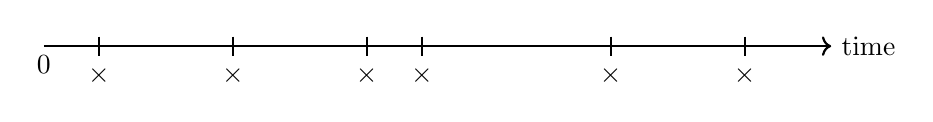
\begin{tikzpicture}
\draw[->, thick] (0,0) -- (10,0) node[right] {time};
\foreach \x in {0.7,2.4,4.1,4.8,7.2,8.9}
  \draw[thick] (\x,0.12) -- (\x,-0.12) node[below] {$\times$};
\node[below] at (0,0) {$0$};
\end{tikzpicture}
\end{center}

\textbf{Analogy.} A Poisson process is like raindrops hitting a roof at random times. We cannot predict exactly when the next drop arrives, but we can describe the average rate and the probability of counts over time intervals.

\section{Exponential Waiting Times}

If the events follow a Poisson process with rate $\lambda$, then the waiting time until the first event is exponential:
\[
T_1\sim \operatorname{Exponential}(\lambda).
\]

The density is
\[
f(t)=\lambda e^{-\lambda t},
\qquad t\geq 0.
\]

The distribution function is
\[
F(t)=\Prob(T_1\leq t)=1-e^{-\lambda t}.
\]

Therefore,
\[
\Prob(T_1>t)=e^{-\lambda t}.
\]

The expected waiting time is
\[
\E[T_1]=\frac1{\lambda}.
\]

\begin{remark}
Some books parameterize the exponential distribution using the mean instead of the rate. In this course, when we write $\operatorname{Exponential}(\lambda)$ for a Poisson process, $\lambda$ is the rate and the mean is $1/\lambda$.
\end{remark}

\section{Deriving the Poisson Count Distribution}

Let
\[
T_1,T_2,\ldots
\]
be independent exponential waiting times with rate $\lambda$.

Let
\[
S_k=T_1+\cdots+T_k
\]
be the time of the $k$th event.

The event
\[
N(t)=k
\]
means:
\[
S_k\leq t
\quad\text{and}\quad
S_{k+1}>t.
\]

So
\[
\Prob(N(t)=k)
=
\Prob(S_k\leq t)-\Prob(S_{k+1}\leq t).
\]

Using the gamma distribution for $S_k$, this leads to
\[
\Prob(N(t)=k)=e^{-\lambda t}\frac{(\lambda t)^k}{k!}.
\]

\section{Earthquake Example}

\begin{example}
Earthquakes in a region occur according to a Poisson process with an average of 104 earthquakes per year.

Find the probability that:
\begin{enumerate}[label=(\alph*)]
    \item a given week has at most one earthquake,
    \item three consecutive earthquakes are at least one week apart from each other,
    \item a week with two earthquakes has them on different days.
\end{enumerate}
\end{example}

\begin{answer}
Since there are 104 earthquakes per year, the average number per week is
\[
\lambda=\frac{104}{52}=2.
\]
So for one week,
\[
N\sim \operatorname{Poisson}(2).
\]

\textbf{(a)} At most one earthquake means
\[
N\leq 1.
\]
Thus,
\[
\Prob(N\leq 1)=\Prob(N=0)+\Prob(N=1).
\]
Using the Poisson formula,
\[
\Prob(N=0)=e^{-2},
\]
and
\[
\Prob(N=1)=e^{-2}\frac{2^1}{1!}=2e^{-2}.
\]
Therefore,
\[
\Prob(N\leq 1)=3e^{-2}\approx 0.406.
\]

\textbf{(b)} The waiting times between earthquakes are independent exponential random variables with rate 2 per week:
\[
T_1,T_2\sim \operatorname{Exponential}(2).
\]

Three consecutive earthquakes are at least one week apart if the two gaps between them are both greater than 1:
\[
T_1>1
\quad\text{and}\quad
T_2>1.
\]

Since $T_1$ and $T_2$ are independent,
\[
\Prob(T_1>1,T_2>1)
=
\Prob(T_1>1)\Prob(T_2>1).
\]
For an exponential random variable,
\[
\Prob(T>1)=e^{-2}.
\]
Therefore,
\[
\Prob(T_1>1,T_2>1)
=
e^{-2}e^{-2}
=
e^{-4}.
\]

\textbf{(c)} Given that two earthquakes occur in a week, their locations within the week behave like two independent random points uniformly distributed over the week.

Take the day of one earthquake. The probability that the other earthquake falls on the same day is
\[
\frac17.
\]
Therefore, the probability that it falls on a different day is
\[
1-\frac17=\frac67.
\]

Hence,
\[
\Prob(\text{different days}\mid \text{two earthquakes in a week})=\frac67.
\]
\end{answer}

\section{Thinning of a Poisson Process}

Suppose events occur according to a Poisson process with rate $\lambda$. Each event is observed with probability $p$, independently of all other events.

Then:
\begin{itemize}[leftmargin=1.2cm]
    \item observed events form a Poisson process with rate $\lambda p$,
    \item unobserved events form a Poisson process with rate $\lambda(1-p)$,
    \item the observed and unobserved processes are independent.
\end{itemize}

\begin{proposition}[Thinning]
If a Poisson process with rate $\lambda$ is thinned by independently keeping each point with probability $p$, then the retained process is a Poisson process with rate $\lambda p$.
\end{proposition}

\textbf{Analogy.} Imagine a stream of phone calls. If each call has probability $p$ of being answered, the answered calls still arrive according to a Poisson process, but with a smaller rate.

\section{Major and Minor Earthquakes}

\begin{example}
Earthquakes occur on average twice a week. Each earthquake is major with probability $0.01$ and minor otherwise.

\begin{enumerate}[label=(\alph*)]
    \item What is the probability that there are no major earthquakes in a given year?
    \item What is the probability that there are no major earthquakes and at least one minor earthquake in a given week?
\end{enumerate}
\end{example}

\begin{answer}
\textbf{(a)} The total earthquake rate is
\[
2\text{ per week}.
\]
In one year,
\[
2\times 52=104
\]
earthquakes are expected.

Major earthquakes occur with probability $0.01$. By thinning, major earthquakes form a Poisson process with yearly mean
\[
104(0.01)=1.04.
\]

Let
\[
X=\text{number of major earthquakes in a year}.
\]
Then
\[
X\sim \operatorname{Poisson}(1.04).
\]

Thus,
\[
\Prob(X=0)=e^{-1.04}\approx 0.35.
\]

\textbf{(b)} In one week, the major earthquake rate is
\[
2(0.01)=0.02.
\]
Let
\[
X=\text{number of major earthquakes in a week}.
\]
Then
\[
X\sim \operatorname{Poisson}(0.02).
\]

The minor earthquake rate is
\[
2(0.99)=1.98.
\]
Let
\[
Y=\text{number of minor earthquakes in a week}.
\]
Then
\[
Y\sim \operatorname{Poisson}(1.98).
\]

By thinning, $X$ and $Y$ are independent.

We need
\[
\Prob(X=0,Y>0).
\]
Using independence,
\[
\Prob(X=0,Y>0)=\Prob(X=0)\Prob(Y>0).
\]

Now,
\[
\Prob(X=0)=e^{-0.02}.
\]
Also,
\[
\Prob(Y>0)=1-\Prob(Y=0)=1-e^{-1.98}.
\]

Therefore,
\[
\Prob(X=0,Y>0)=e^{-0.02}(1-e^{-1.98})\approx 0.84.
\]
\end{answer}

\section{Superposition of Poisson Processes}

Superposition means adding independent Poisson processes together.

\begin{proposition}[Superposition]
If two independent Poisson processes have rates $\lambda_1$ and $\lambda_2$, then their combined process is a Poisson process with rate
\[
\lambda_1+\lambda_2.
\]
\end{proposition}

\textbf{Analogy.} If northbound cars pass at rate 3 per minute and southbound cars pass at rate 2 per minute, then all cars together pass at rate 5 per minute.

\section{Traffic Accidents Example}

\begin{example}
Traffic accidents in a town occur according to a Poisson process at a rate of two accidents per week.

\begin{enumerate}[label=(\alph*)]
    \item What is the probability that a given day has no accidents?
    \item Whenever there is an accident, the risk is 1 in 10 that it will cause personal injury. What is the probability that a given month has at least one such accident?
    \item Let $N$ be the number of accident-free weeks in a year. What is the distribution of $N$?
\end{enumerate}
\end{example}

\begin{answer}
\textbf{(a)} The accident rate is 2 per week. For one day,
\[
\lambda=\frac27.
\]
Thus,
\[
\Prob(\text{no accidents in a day})
=
e^{-2/7}.
\]

\textbf{(b)} Personal-injury accidents are obtained by thinning. Each accident causes personal injury with probability
\[
\frac1{10}.
\]
So the rate of personal-injury accidents is
\[
2\cdot\frac1{10}=0.2
\]
per week.

Assuming 4 weeks per month, the monthly mean is
\[
0.2(4)=0.8.
\]

Let
\[
X=\text{number of personal-injury accidents in a month}.
\]
Then
\[
X\sim \operatorname{Poisson}(0.8).
\]

We need
\[
\Prob(X\geq 1).
\]
Thus,
\[
\Prob(X\geq1)=1-\Prob(X=0)=1-e^{-0.8}.
\]

\textbf{(c)} A week is accident-free if it has zero accidents. Since accidents occur at rate 2 per week,
\[
\Prob(\text{a week is accident-free})=e^{-2}.
\]

There are 52 weeks in a year. Let
\[
N=\text{number of accident-free weeks in a year}.
\]
Each week is classified as accident-free or not accident-free. Hence
\[
N\sim \operatorname{Binomial}(52,e^{-2}).
\]
\end{answer}

\section{Two-Direction Car Process}

\begin{example}
Southbound and northbound cars pass a point on a rural highway according to two independent Poisson processes, at rates 2 and 3 cars per minute, respectively.

\begin{enumerate}[label=(\alph*)]
    \item What is the probability that exactly two cars pass in a given minute?
    \item What is the probability that exactly one northbound car and one southbound car pass in a given minute?
    \item If two cars pass in a minute, what is the probability that they are both northbound?
    \item If four cars pass between 11:55 am and 12:05 pm, what is the probability that two pass before noon and two after noon?
\end{enumerate}
\end{example}

\begin{answer}
Let
\[
S=\text{number of southbound cars in one minute},
\]
and
\[
N=\text{number of northbound cars in one minute}.
\]

Then
\[
S\sim \operatorname{Poisson}(2),
\qquad
N\sim \operatorname{Poisson}(3),
\]
and they are independent.

\textbf{(a)} By superposition,
\[
S+N\sim \operatorname{Poisson}(2+3)=\operatorname{Poisson}(5).
\]
Therefore,
\[
\Prob(S+N=2)=e^{-5}\frac{5^2}{2!}.
\]

\textbf{(b)} Since $S$ and $N$ are independent,
\[
\Prob(N=1,S=1)=\Prob(N=1)\Prob(S=1).
\]
Thus,
\[
\Prob(N=1,S=1)
=
\left(e^{-3}\frac{3^1}{1!}\right)
\left(e^{-2}\frac{2^1}{1!}\right)
=
6e^{-5}.
\]

\textbf{(c)} We need
\[
\Prob(N=2\mid S+N=2).
\]
By thinning/superposition, given that a total car is observed, it is northbound with probability
\[
\frac{3}{2+3}=\frac35.
\]
Given that two total cars pass, the number that are northbound is
\[
\operatorname{Binomial}\left(2,\frac35\right).
\]
Therefore,
\[
\Prob(\text{both northbound}\mid S+N=2)
=
\left(\frac35\right)^2
=
\frac9{25}.
\]

\textbf{(d)} The interval from 11:55 to 12:05 has length 10 minutes. Given that four cars pass in this 10-minute interval, the event times are uniformly distributed over the interval.

The interval is split into two equal 5-minute parts:
\[
11{:}55\text{ to }12{:}00,
\qquad
12{:}00\text{ to }12{:}05.
\]

Each of the four cars independently has probability
\[
\frac12
\]
of falling before noon.

Thus, the number before noon is
\[
\operatorname{Binomial}\left(4,\frac12\right).
\]

Therefore,
\[
\Prob(\text{two before noon and two after})
=
\binom42\left(\frac12\right)^2\left(\frac12\right)^2
=
\frac{6}{16}
=
\frac38.
\]
\end{answer}

\section{Overlapping Interval Example}

\begin{example}
Consider a Poisson process with rate $\lambda$.

\begin{enumerate}[label=(\alph*)]
    \item Compute the probability that the 10th event occurs 2 or more time units after the 9th event.
    \item Compute the probability of 2 events in $[1,4]$ and 3 events in $[3,5]$.
\end{enumerate}
\end{example}

\begin{answer}
\textbf{(a)} The time between the 9th and 10th events is an interarrival time:
\[
T_{10}=S_{10}-S_9.
\]
For a Poisson process,
\[
T_{10}\sim \operatorname{Exponential}(\lambda).
\]
Therefore,
\[
\Prob(T_{10}\geq2)=e^{-2\lambda}.
\]

\textbf{(b)} The intervals $[1,4]$ and $[3,5]$ overlap. Break them into disjoint intervals:
\[
[1,3],\qquad [3,4],\qquad [4,5].
\]

Let
\[
A=N([1,3]),\qquad B=N([3,4]),\qquad C=N([4,5]).
\]

Then
\[
A\sim \operatorname{Poisson}(2\lambda),
\]
\[
B\sim \operatorname{Poisson}(\lambda),
\]
\[
C\sim \operatorname{Poisson}(\lambda),
\]
and $A,B,C$ are independent.

The condition
\[
N([1,4])=2
\]
means
\[
A+B=2.
\]

The condition
\[
N([3,5])=3
\]
means
\[
B+C=3.
\]

Possible values of $B$ are
\[
B=0,1,2.
\]

Therefore,
\[
\Prob(N([1,4])=2,\ N([3,5])=3)
\]
\[
=
\sum_{b=0}^{2}\Prob(A=2-b)\Prob(B=b)\Prob(C=3-b).
\]

Using the Poisson formula:
\[
=
\sum_{b=0}^{2}
\left(e^{-2\lambda}\frac{(2\lambda)^{2-b}}{(2-b)!}\right)
\left(e^{-\lambda}\frac{\lambda^b}{b!}\right)
\left(e^{-\lambda}\frac{\lambda^{3-b}}{(3-b)!}\right).
\]
\end{answer}

\section{Customer Arrival Example}

\begin{example}
Customers arrive at a store at rate 10 per hour. Each customer is male or female with probability $1/2$. Suppose exactly 10 women entered during one hour.

\begin{enumerate}[label=(\alph*)]
    \item Compute the probability that exactly 10 men also entered.
    \item Compute the probability that at least 20 customers have entered.
\end{enumerate}
\end{example}

\begin{answer}
By thinning, male and female arrivals are independent Poisson processes with rates
\[
10\cdot\frac12=5
\]
per hour.

Let
\[
M=\text{number of men in the hour},
\qquad
F=\text{number of women in the hour}.
\]
Then
\[
M\sim \operatorname{Poisson}(5),
\qquad
F\sim \operatorname{Poisson}(5),
\]
and $M$ and $F$ are independent.

We are given
\[
F=10.
\]
Since $M$ and $F$ are independent, this information does not change the distribution of $M$.

\textbf{(a)}
\[
\Prob(M=10\mid F=10)=\Prob(M=10)
=
e^{-5}\frac{5^{10}}{10!}.
\]

\textbf{(b)} At least 20 customers have entered means
\[
M+F\geq20.
\]
Given that
\[
F=10,
\]
this is equivalent to
\[
M+10\geq20,
\]
so
\[
M\geq10.
\]

Therefore,
\[
\Prob(M+F\geq20\mid F=10)
=
\Prob(M\geq10).
\]

Since
\[
M\sim \operatorname{Poisson}(5),
\]
we get
\[
\Prob(M\geq10)
=
\sum_{j=10}^{\infty}e^{-5}\frac{5^j}{j!}
=
1-\sum_{j=0}^{9}e^{-5}\frac{5^j}{j!}.
\]
\end{answer}

\section{Summary}

\begin{itemize}[leftmargin=1.2cm]
    \item A Poisson process models randomly occurring events in continuous time.
    \item If the process has rate $\lambda$, then
    \[
    N(t)\sim \operatorname{Poisson}(\lambda t).
    \]
    \item The Poisson probability formula is
    \[
    \Prob(N(t)=k)=e^{-\lambda t}\frac{(\lambda t)^k}{k!}.
    \]
    \item Interarrival times in a Poisson process are independent exponential random variables with rate $\lambda$.
    \item The exponential survival probability is
    \[
    \Prob(T>t)=e^{-\lambda t}.
    \]
    \item Thinning a Poisson process with probability $p$ gives a new Poisson process with rate $\lambda p$.
    \item The thinned observed and unobserved processes are independent.
    \item Superposition of independent Poisson processes adds the rates.
    \item For overlapping intervals, break the intervals into disjoint pieces.
    \item For branching processes, extinction probability is found by solving $s=G(s)$ and taking the smallest solution in $[0,1]$.
\end{itemize}

\section{Essay-Type Questions}

\begin{enumerate}[label=\textbf{Q\arabic*.}, leftmargin=1.2cm]
    \item Explain how the disease spread example can be modelled as a branching process.
    \item Define a Poisson process and state the distribution of $N(t)$.
    \item Explain the relationship between Poisson processes and exponential waiting times.
    \item Derive the formula for $\Prob(N(t)=k)$ using arrival times $S_k$.
    \item Explain thinning of a Poisson process with an example.
    \item Explain superposition of independent Poisson processes with an example.
    \item In a Poisson process, explain how to handle overlapping intervals.
    \item Solve the traffic accident example using thinning and Poisson probabilities.
\end{enumerate}

\section{Answers to Essay-Type Questions}

\subsection*{Answer 1}

The disease spread can be modelled as a branching process because each infected individual produces a random number of new infected individuals. These new infections form the next generation. If $Z_n$ is the number of infected individuals on day $n$, then $Z_{n+1}$ is formed by adding the new infections caused by all individuals in generation $n$.

If each person contacts a Poisson number of people with mean 10 and each contact becomes infected with probability $p$, then the number of new infections caused by one infected person is Poisson with mean $10p$. Thus the offspring mean is $\mu=10p$.

\subsection*{Answer 2}

A Poisson process is a point process where the waiting times between consecutive events are independent exponential random variables with rate $\lambda$.

If $N(t)$ is the number of events in time interval $[0,t]$, then
\[
N(t)\sim \operatorname{Poisson}(\lambda t).
\]
Therefore,
\[
\Prob(N(t)=k)=e^{-\lambda t}\frac{(\lambda t)^k}{k!}.
\]

\subsection*{Answer 3}

In a Poisson process with rate $\lambda$, the waiting time until the first event is exponential with rate $\lambda$:
\[
T_1\sim \operatorname{Exponential}(\lambda).
\]
Also, all interarrival times are independent and identically distributed:
\[
T_1,T_2,\ldots \sim \operatorname{Exponential}(\lambda).
\]
Thus the Poisson process describes counts over time, while the exponential distribution describes the waiting time between events.

\subsection*{Answer 4}

Let $S_k$ be the time of the $k$th event. The event $N(t)=k$ means that the $k$th event occurred before time $t$, but the $(k+1)$th event occurred after time $t$:
\[
S_k\leq t<S_{k+1}.
\]
Thus,
\[
\Prob(N(t)=k)=\Prob(S_k\leq t)-\Prob(S_{k+1}\leq t).
\]
Using the gamma distribution of $S_k$, this simplifies to
\[
\Prob(N(t)=k)=e^{-\lambda t}\frac{(\lambda t)^k}{k!}.
\]

\subsection*{Answer 5}

Thinning means keeping each point of a Poisson process independently with probability $p$. If the original process has rate $\lambda$, then the retained process has rate $\lambda p$.

For example, if accidents occur at rate 2 per week and each accident causes personal injury with probability $1/10$, then personal-injury accidents form a Poisson process with rate
\[
2\cdot\frac1{10}=0.2
\]
per week.

\subsection*{Answer 6}

Superposition means combining independent Poisson processes. If two independent processes have rates $\lambda_1$ and $\lambda_2$, then their combined process has rate
\[
\lambda_1+\lambda_2.
\]

For example, if northbound cars arrive at rate 3 per minute and southbound cars arrive at rate 2 per minute, then all cars together arrive at rate
\[
3+2=5
\]
per minute.

\subsection*{Answer 7}

For overlapping intervals, first split the time line into disjoint intervals. Counts in disjoint intervals of a Poisson process are independent.

For example, to study counts in $[1,4]$ and $[3,5]$, split into
\[
[1,3],\quad [3,4],\quad [4,5].
\]
Then write the conditions using the counts in these disjoint pieces.

\subsection*{Answer 8}

Traffic accidents occur at rate 2 per week.

For one day, the rate is
\[
\frac27.
\]
So the probability of no accidents in one day is
\[
e^{-2/7}.
\]

Personal-injury accidents are obtained by thinning with probability $1/10$. Therefore the personal-injury accident rate is
\[
2\cdot\frac1{10}=0.2
\]
per week. For a 4-week month, the mean is
\[
0.8.
\]
Thus the probability of at least one personal-injury accident in a month is
\[
1-e^{-0.8}.
\]

For accident-free weeks, a week has zero accidents with probability
\[
e^{-2}.
\]
Therefore, if $N$ is the number of accident-free weeks in a year,
\[
N\sim \operatorname{Binomial}(52,e^{-2}).
\]

\end{document}
